
\begin{figure}
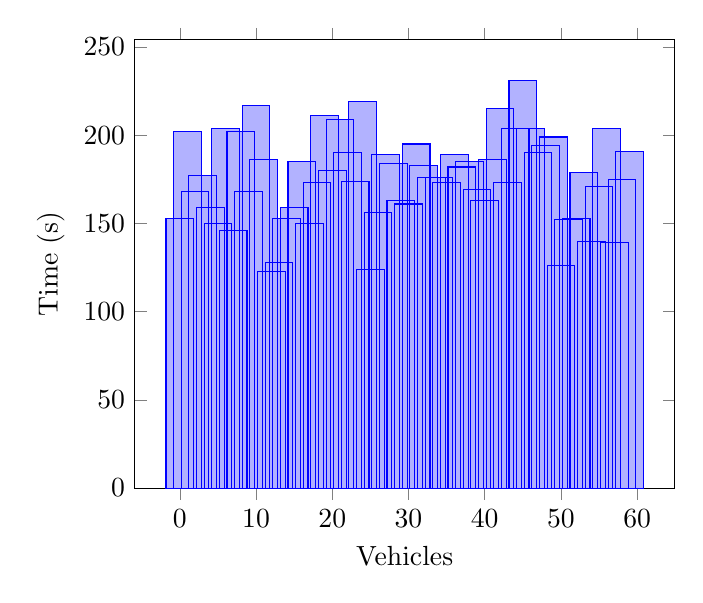
\begin{tikzpicture}
\begin{axis}[
legend style={anchor=west},
xlabel=Vehicles,
ylabel=Time (s),
ymin=0,
ybar,
]
\addplot coordinates {
(0, 153)
(1, 202)
(2, 168)
(3, 177)
(4, 159)
(5, 150)
(6, 204)
(7, 146)
(8, 202)
(9, 168)
(10, 217)
(11, 186)
(12, 123)
(13, 128)
(14, 153)
(15, 159)
(16, 185)
(17, 150)
(18, 173)
(19, 211)
(20, 180)
(21, 209)
(22, 190)
(23, 174)
(24, 219)
(25, 124)
(26, 156)
(27, 189)
(28, 184)
(29, 163)
(30, 161)
(31, 195)
(32, 183)
(33, 176)
(34, 176)
(35, 173)
(36, 189)
(37, 182)
(38, 185)
(39, 169)
(40, 163)
(41, 186)
(42, 215)
(43, 173)
(44, 204)
(45, 231)
(46, 204)
(47, 190)
(48, 194)
(49, 199)
(50, 126)
(51, 152)
(52, 153)
(53, 179)
(54, 140)
(55, 171)
(56, 204)
(57, 139)
(58, 175)
(59, 191)
};

\end{axis}
\end{tikzpicture}
\label{tik:0:3_V, 3_V.-60, 4_S, 5_S, 5_S.-30, 7_S, 7_S.-25, 11_S, 11_S.-50, 13_S, 15_N, 17_S, 17_S.-60, 18_S}
\caption{0 percent diving with GSC on route $3_V, 3_V.-60, 4_S, 5_S, 5_S.-30, 7_S, 7_S.-25, 11_S, 11_S.-50, 13_S, 15_N, 17_S, 17_S.-60, 18_S$}
\end{figure}
